\section{Análise exploratória}

As classes são razoavelmente balanceadas (Tabela~\ref{tab:classes}): responder sempre EGFR, a majoritária, acerta 29,3\%, e esse é o piso de comparação do restante do trabalho. A Figura~\ref{fig:boxplots} mostra os cinco descritores por alvo. DRD2 se destaca por TPSA e HBD baixos (mediana de 54,5~\AA$^2$ e 1 doador, contra 98 a 101~\AA$^2$ nos demais alvos), o que é compatível com ligantes de receptores cerebrais, em geral pouco polares. EGFR reúne as moléculas mais pesadas e lipofílicas (mediana de 497,6~Da e LogP de 4,6). HDAC1 tem o maior HBD (mediana 3), em linha com o grupo hidroxamato presente em muitos inibidores dessa enzima. BACE1 e HDAC1 se sobrepõem em massa, TPSA e HBA.

\begin{figure}[ht]
\centering
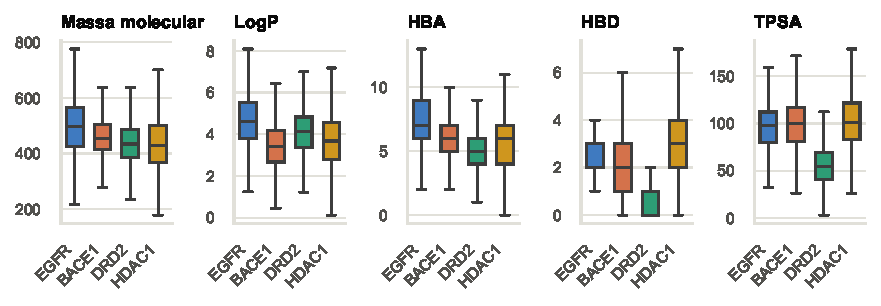
\includegraphics[width=\textwidth]{figures/feature_boxplots.pdf}
\caption{Descritores por proteína-alvo. Caixas mostram os quartis e as hastes 1,5 vez a amplitude interquartil; valores extremos foram omitidos.}
\label{fig:boxplots}
\end{figure}

TPSA, HBA e HBD são correlacionadas entre si (Spearman de 0,72 entre TPSA e HBA e de 0,69 entre TPSA e HBD), pois as três medem polaridade. Isso não prejudica a árvore, mas divide a importância entre elas. No plano LogP $\times$ TPSA (Figura~\ref{fig:scatter}), DRD2 se concentra em TPSA baixa e EGFR em LogP alto, enquanto BACE1 e HDAC1 ocupam a mesma região.

\begin{figure}[ht]
\centering
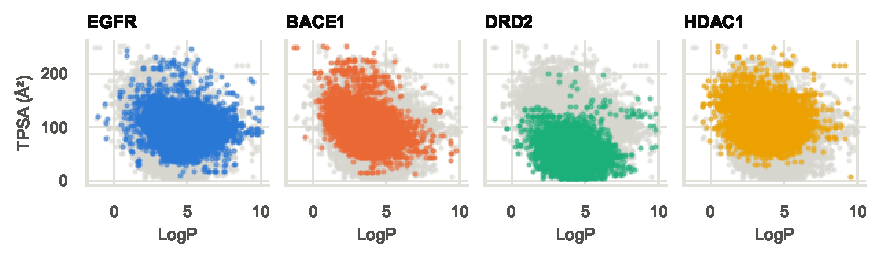
\includegraphics[width=\textwidth]{figures/logp_tpsa_by_class.pdf}
\caption{LogP $\times$ TPSA. Cada painel destaca uma classe sobre todas as moléculas (cinza).}
\label{fig:scatter}
\end{figure}

Nenhum descritor basta sozinho. Uma árvore de profundidade 3 treinada com uma única feature, em validação cruzada de 5 partes, atinge de 37,8\% (massa molecular) a 45,1\% (HBD): todas superam o piso de 29,3\%, mas nenhuma passa de 45\%. A árvore precisa combinar atributos, e o desempenho esperado com só cinco descritores globais é limitado, sobretudo entre BACE1 e HDAC1. Isso motiva as features extraídas do SMILES (Seção~\ref{sec:metodologia}).
